\chapter{Performance Analysis}
%high prio
Performance experiments:

%statistical restrictions, show you are aware of restricitons. what you have tested only once, twice, etc..

\section{Startup time}
% TODO

\begin{figure}[h]
	\centering
	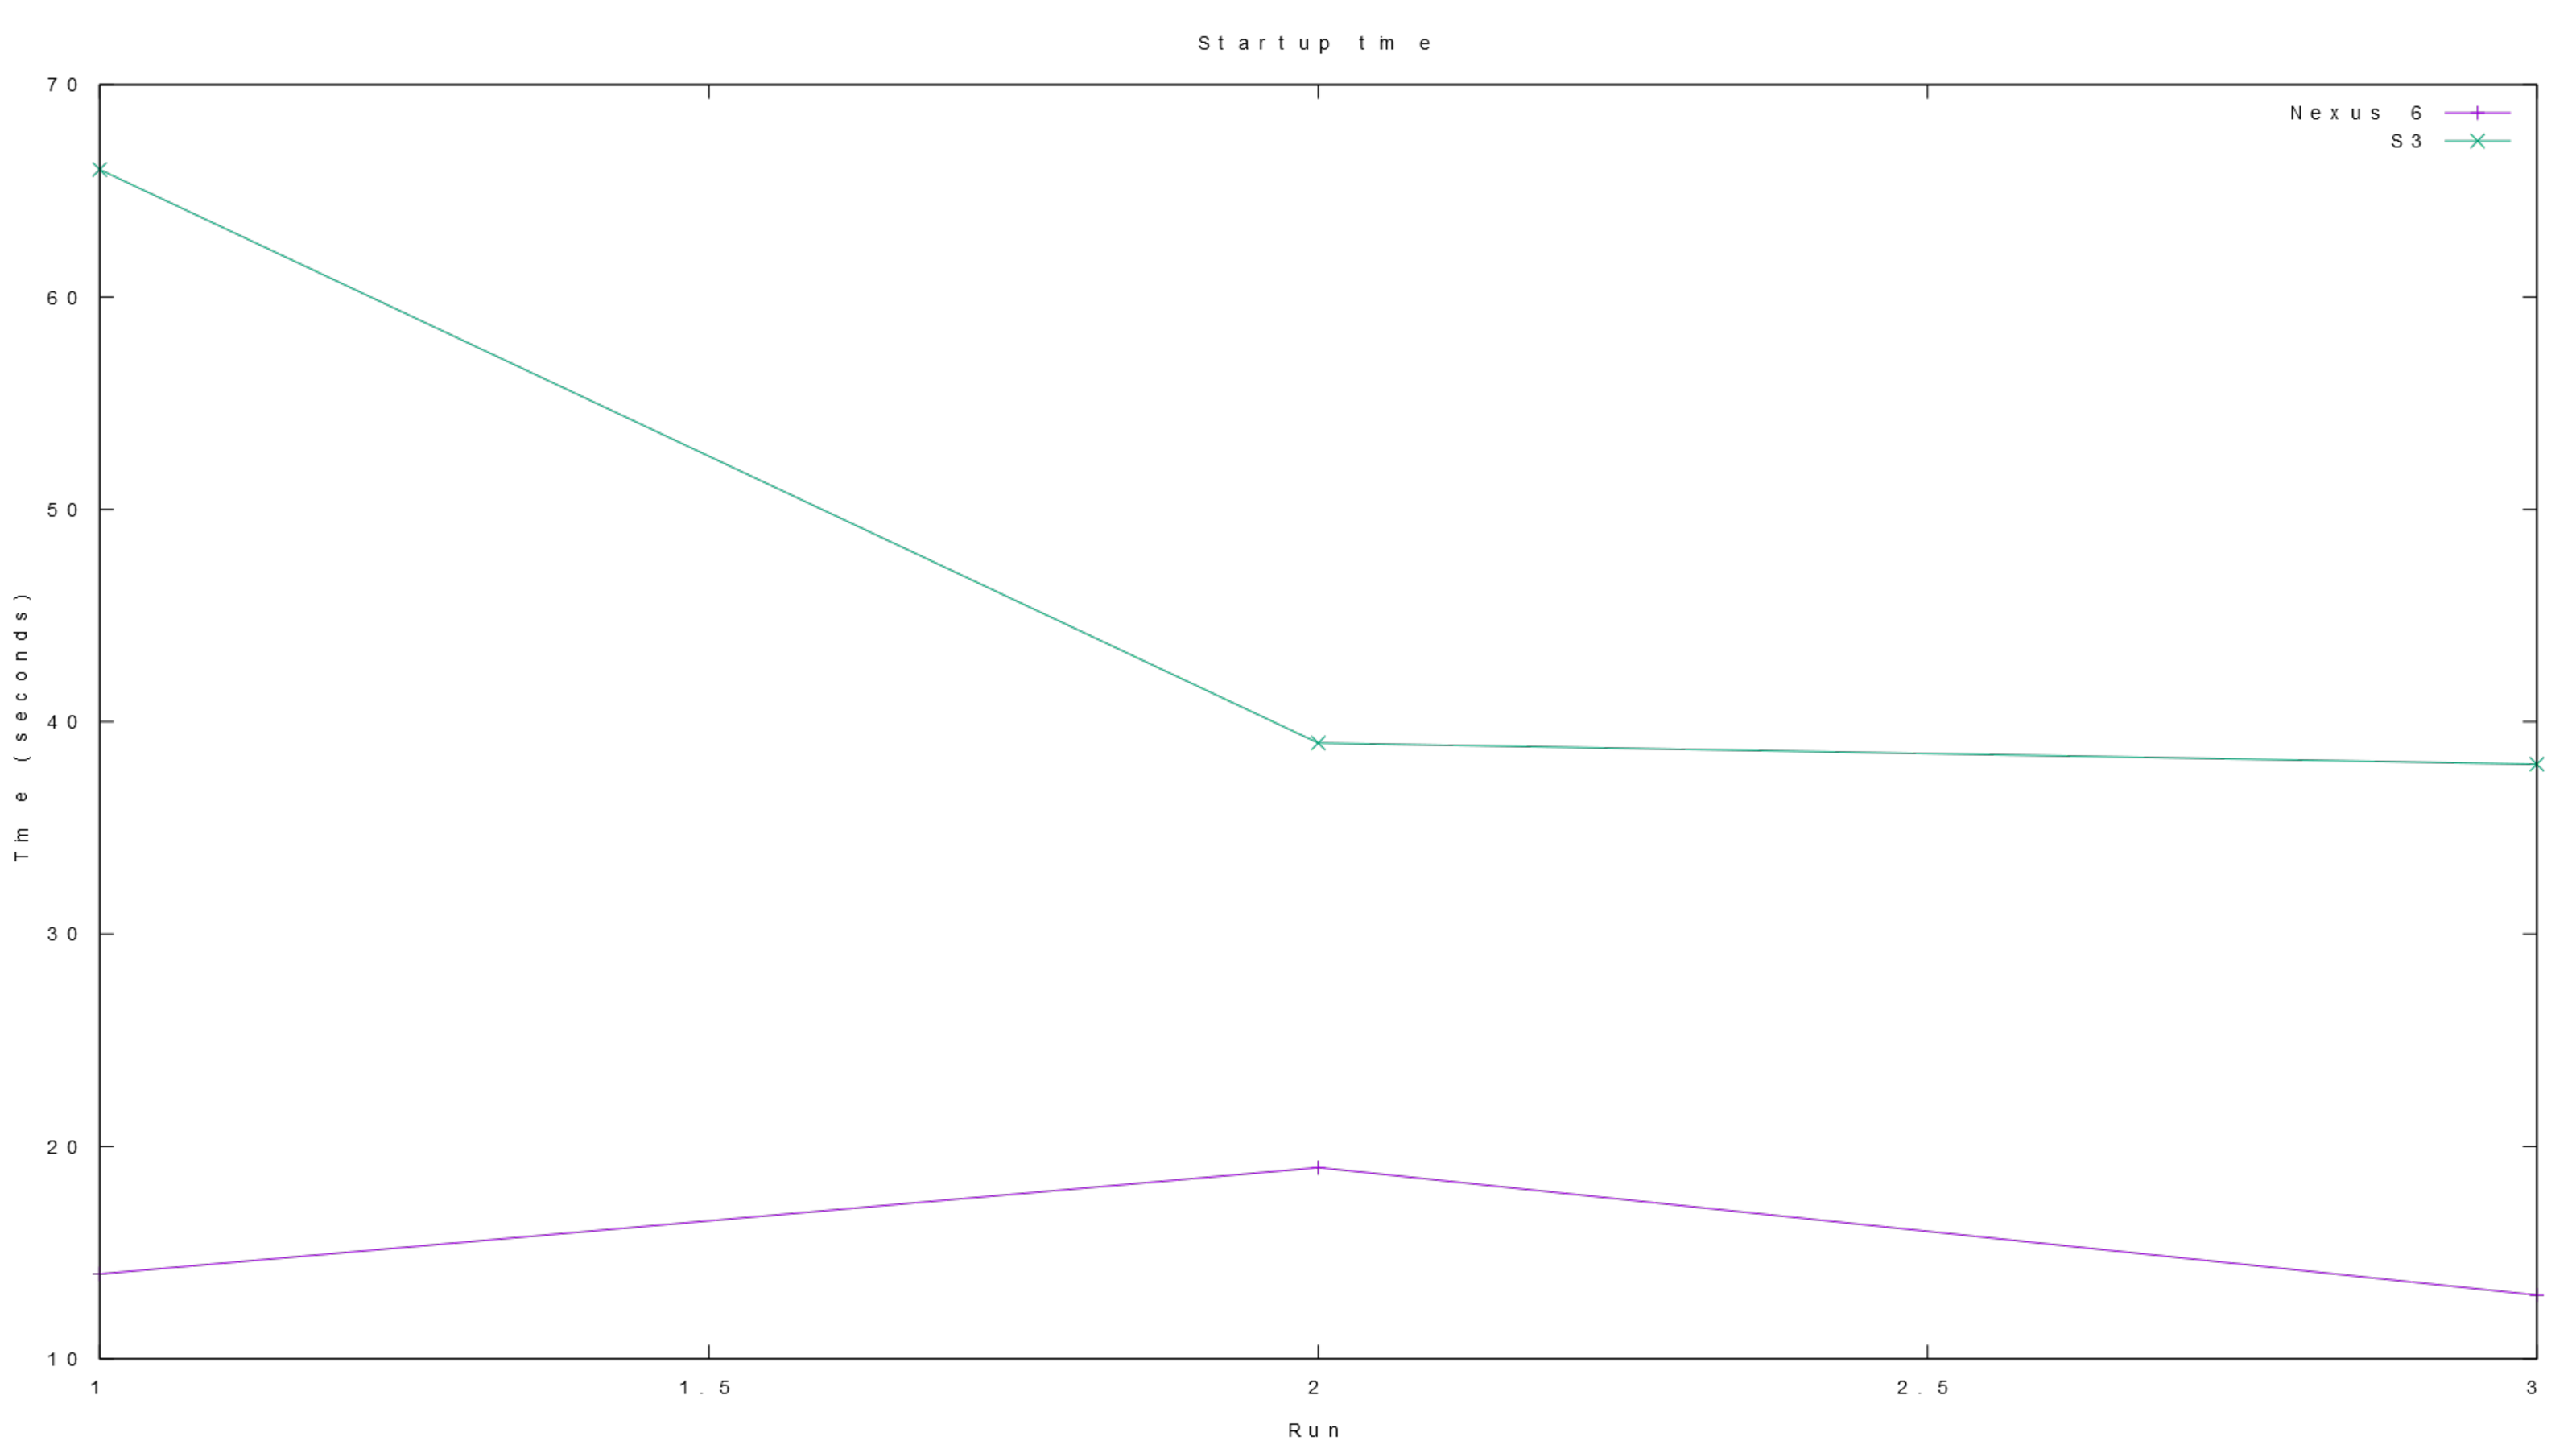
\includegraphics[width=\textwidth]{startup_time}
	\caption{Startup experience}
	\label{fig:startup_time}
\end{figure}

Startup time of Tribler also briefly Youtube (same hardware clean slate). Include log snippits in thesis (code quote style). Real data + graph + text of experiment: what you did and results. Repeat 10-ish time or so for accuracy; on 2 phone models. Graph bar chart with certainty intervals (1 bar Nexus 5, 1 bar Nexus 6). Split: Java GUI, Core started (known variance).



\section{GUI Responose Time}
Latency during first hour, after first hour
What does it say about the design?


\section{Content Discovery Performance}
First discovered content, latency, cdf


\section{Search Performance}

\begin{figure}[h]
	\centering
	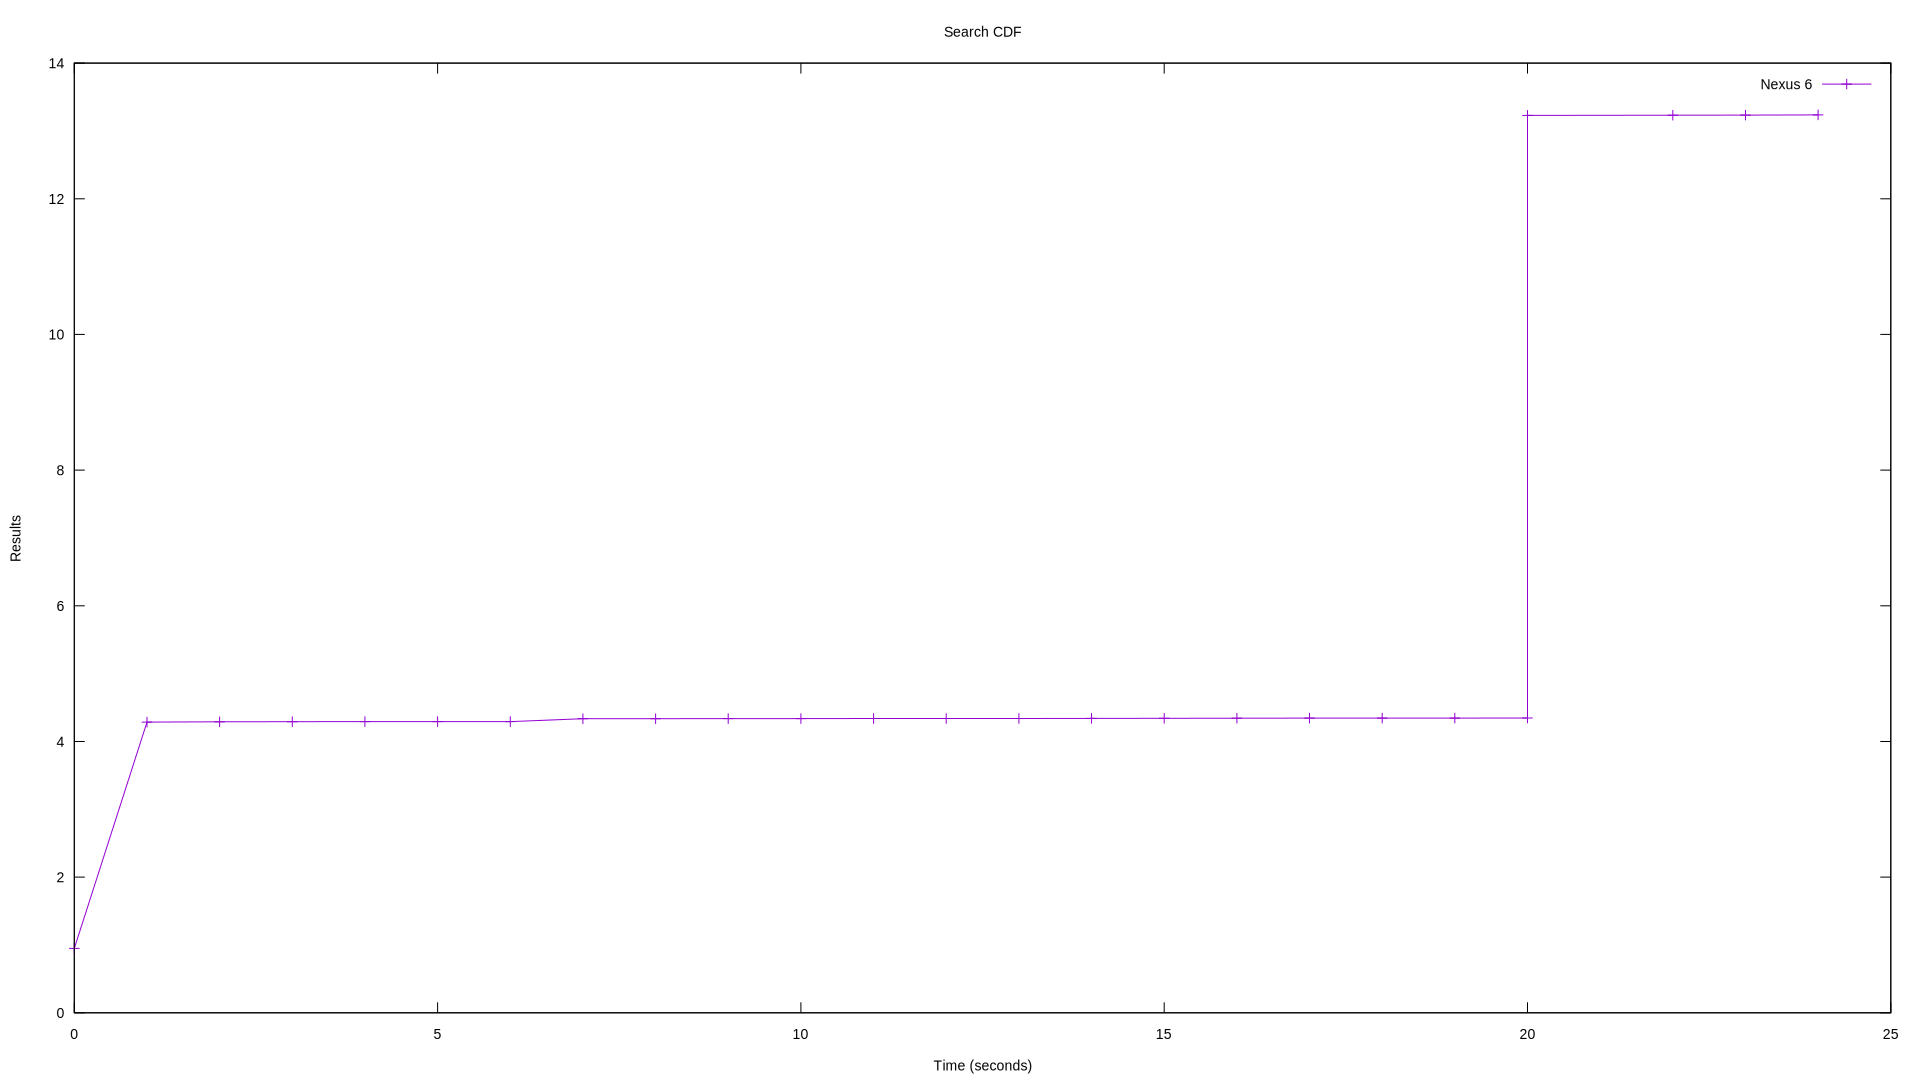
\includegraphics[width=\textwidth]{search_cdf}
	\caption{Search results response time, latency, cdf}
	\label{fig:search_cdf}
\end{figure}


\section{Typical System Load}
y: cpu usage
x: time 0-3 uur

Graph showing cpu and memory consumption from fresh install to an hour idling. 0 tunnels.

Graph showing cpu and memory consumption with max. 10 tunnels after an hour idling.

Graph showing cpu and memory consumption during single download after an hour idling. 0 tunnels.

Graph showing cpu and memory consumption during streaming HD video after an hour idling. 0 tunnels.



stacking of cost, turn all off, turn on one by one or peel off some functionality, look at resulting workload / impact on performace / give relative cost of component


\section{CProfiler Analysis}
Graph showing wall clock time spend on functions running 10 minutes during first half hour with max. 10 tunnels.
flame graph

\begin{figure}[h]
	\centering
	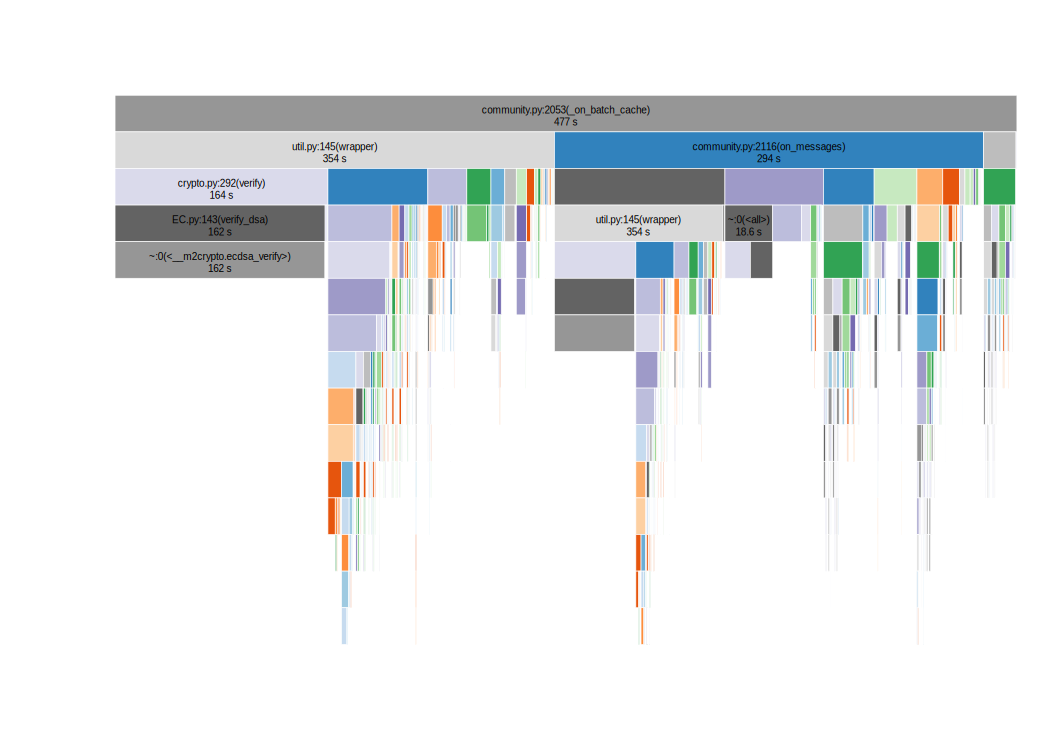
\includegraphics[width=\textwidth]{profile_1468515157}
	\caption{}
	\label{fig:profile_1468515157}
\end{figure}


\section{Test Suite Performance}
Graph showing total run time and average run time per test.

Code coverage?


\section{Multi-chain Scalability Experiment}
%TODO describe multichain experiment

Graph showing scalability or lack thereof of the multi-chain record creation cost.

\begin{figure}[h]
	\centering
	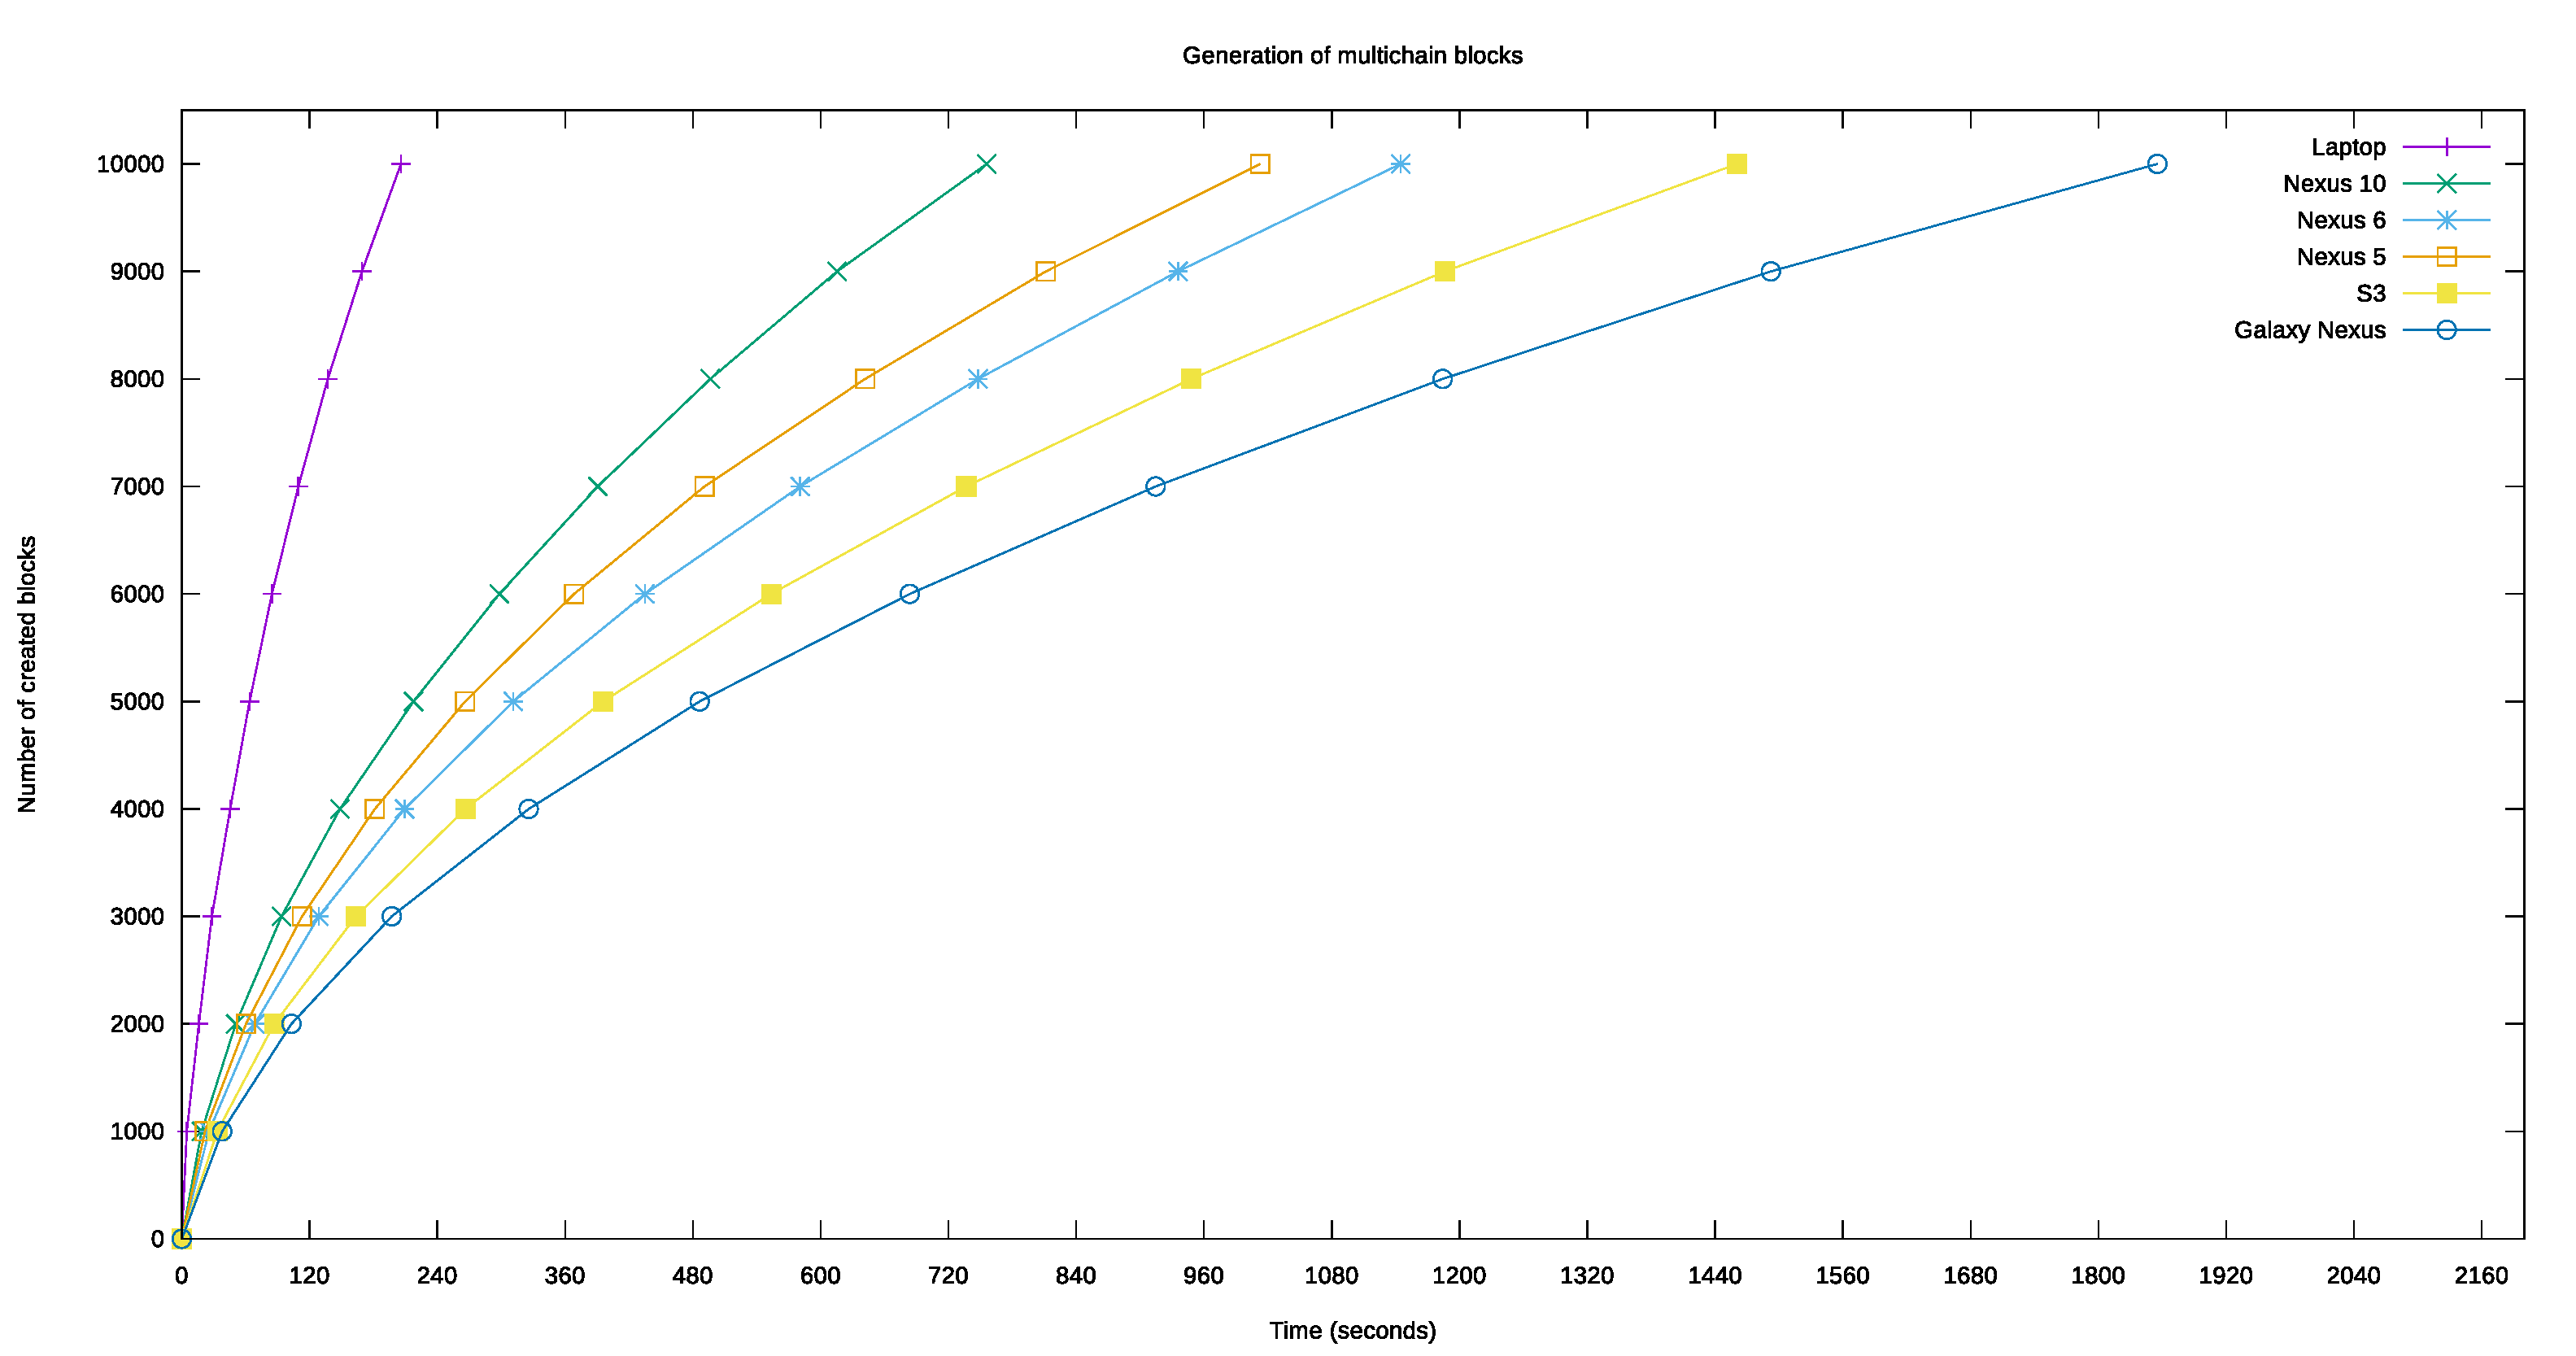
\includegraphics[width=\textwidth]{multichain_scale_3}
	\caption{Multichain record creation cost}
	\label{fig:multichain_scale}
\end{figure}

Clean experiment: no prior exchanges in the database

 


The bandwidth accounting system for the anonymous tunnels, multi-chain, should be capable of holding records on a very large scale.
We conducted an experiment with registering 10.000 blocks between 2 peers, on 5 different models of phones.
Figure \ref{fig:multichain_scale} shows that the curve is not scaling linearly.

The database size appear to have a large impact on the performance. \cite{db_performance}

target: 5 blokjes per 10 minuten

cpu, io

7 transactions Bitcoin, this is higher

decentralized, inherently parallel, 1 transaction per 10 min.

direct signatures vs global consensus


\section{Phone-to-Phone new content discover time}
%TODO

\begin{figure}[h]
	\centering
	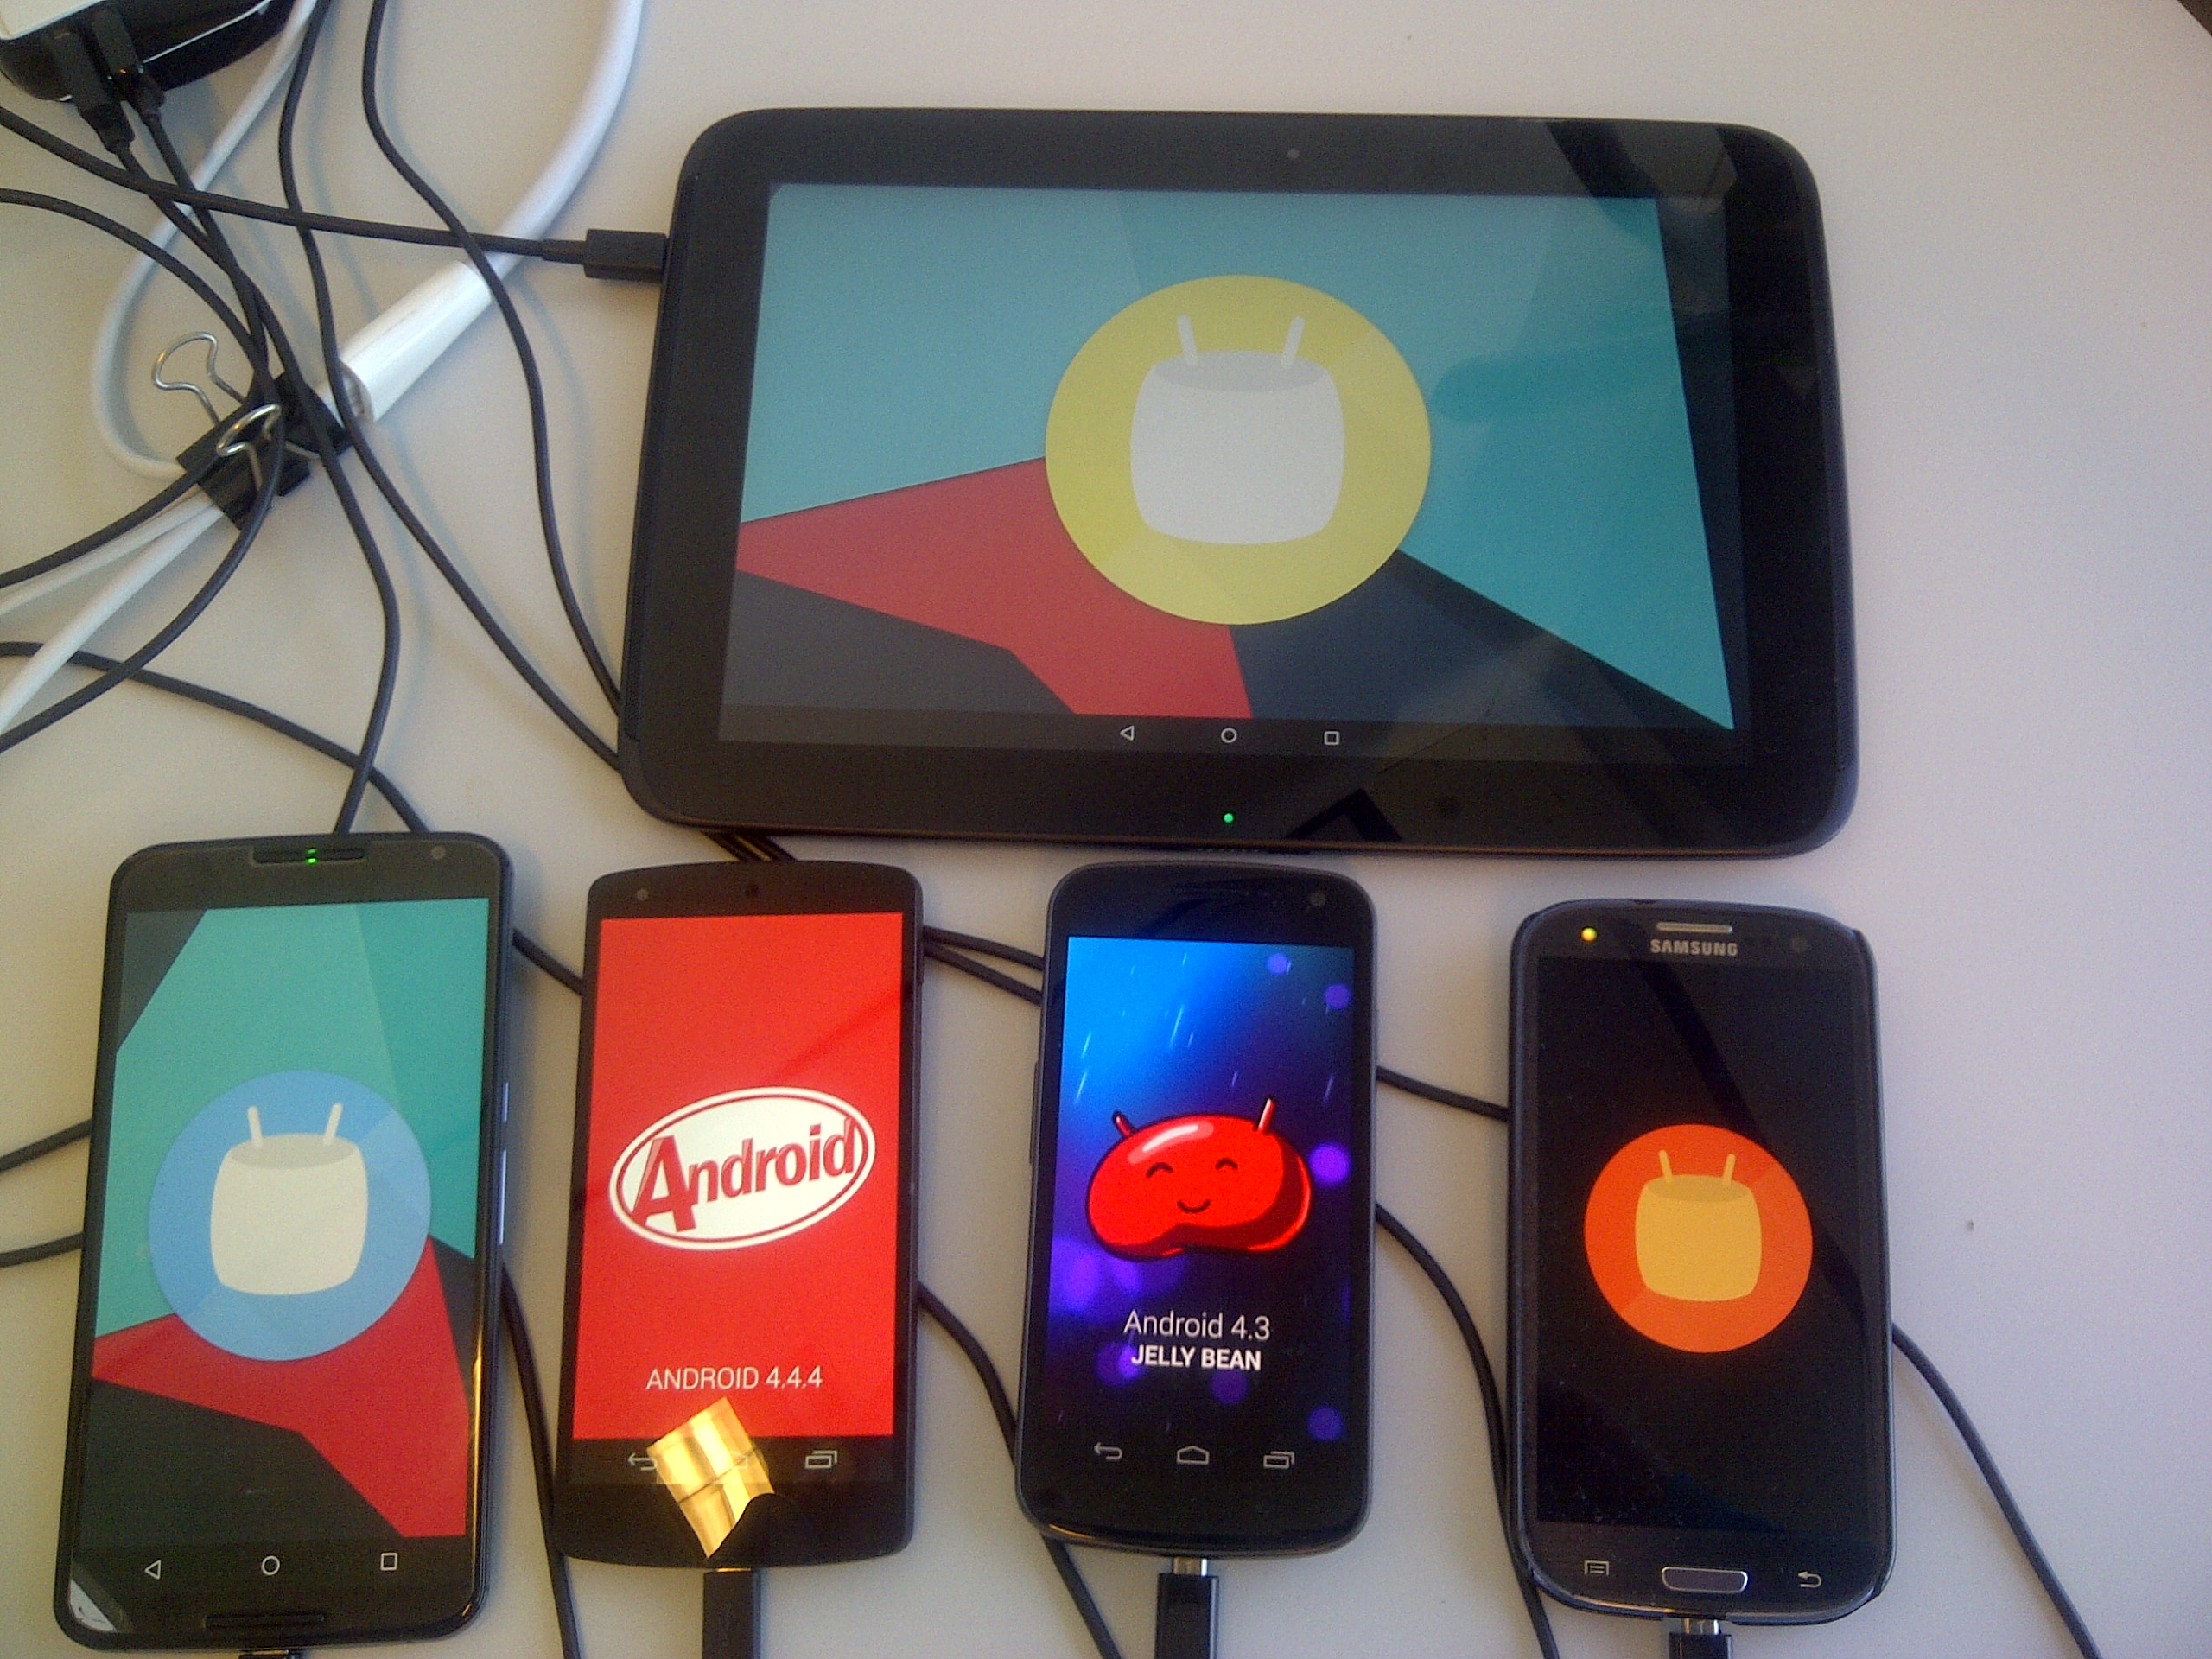
\includegraphics[width=\textwidth]{phones}
	\caption{Experiment setup}
	\label{fig:phones}
\end{figure}

Key experiment: content dissemination experiment with a several phones.

Graph: time on X-axes, Y-axes number of phones which received the content. Timepoint 0: file added at source.

1 phone has channel.
10 phones get subscribed to the same channel
continuously add file to source phone (10+ swarms in seconds)
see them appear at the various screens with a refresh

describe experiment above with content dissemination. 1 photo of the phones "experimental setup".


\section{Transfer time of app}

Bluetooth,
WiFi-direct (P2P wifi)


\section{DAS5 1 to 1000000} 

